
%\subsubsection{Optimizations}







%\noindent
%\textbf{Optimizations:}
\subsubsection{Optimizations}
Notwithstanding the benefits of the FaaS model,
%in the provisioning of computing services, 
the satisfaction of low-latency requirements by a \textit{Serverless Edge Platform} demands further optimizations.

%In the FaaS model
First, functions are externally triggered by HTTP requests. In the context of real-time applications, communication overhead must be kept minimal. As such, the edge platform must include an interface that allows clients to trigger sequential or parallel execution of functions composing different services without the overhead associated to the HTTP protocol. For instance, the \textit{WebSocket protocol}
%\footnote{Documentation available at https://tools.ietf.org/html/rfc6455}
%is a standardized protocol that 
provides full-duplex communication channels over a single TCP connection. %Figure~\ref illustrates this feature.

%For this, each task is deployed as a stateless, fully-managed function and exposed as a web service. 
%Within milliseconds, the fully-managed platform allocates a containerized runtime instance in which the function is first executed, whereas subsequent executions may take advantage of existing instances.
%Dependencies, if any, are described within a package descriptor and made available by the platform.
%Finally, a third function gets detailed information about each POI from a remote database.
%In particular, OpenWhisk is an state-of-art and open source FaaS platform.

The support of an efficient protocol would enable real-time communication between edge devices and platforms. Still, individual function invocation may add significant latency overhead whenever two or more functions form an execution flow. To avoid this overhead, developers would be forced to either chain function calls through hardcoded dependencies, or write coarser and less cohesive functions. In the former case, the chaining of function also imposes a cost overhead, since caller functions are kept waiting.% for other function(s) to return. 

To address latency, design, cost, and resource efficiency concerns, we propose SEPs to be equipped with a \textit{Workflow Service}. This service allows developers to define, through visual or textual programming, a function execution flow.
%starting with the processing of the input sent by a client and finishing with the result sent back to the client. 
Similarly to single functions, workflows are triggered by events (e.g., an external request); at each intermediary step, result from the current function is passed to the next one. 

\begin{figure}[bp]
	\centering
	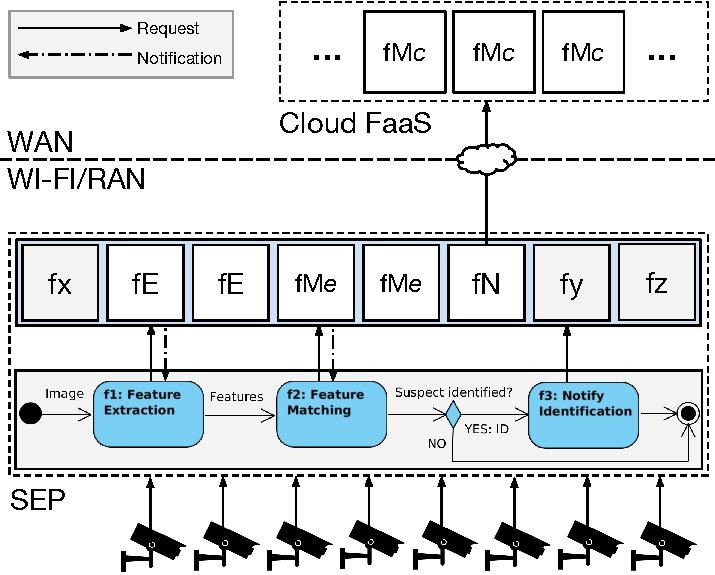
\includegraphics[width=0.97\linewidth]{Figs/Edge_Data_Analytics_Video_Surveillance.pdf}
	\caption{Features from video frames captures by IoT cameras are \textit{extracted} (fE) and, upon positive \textit{matching} (fM$e$), sent for further analysis by a cloud service (fM$c$).}
	\label{fig:Edge_Data_Analytics_Video_Surveillance}
\end{figure}

\begin{figure}[bp]
	\centering
	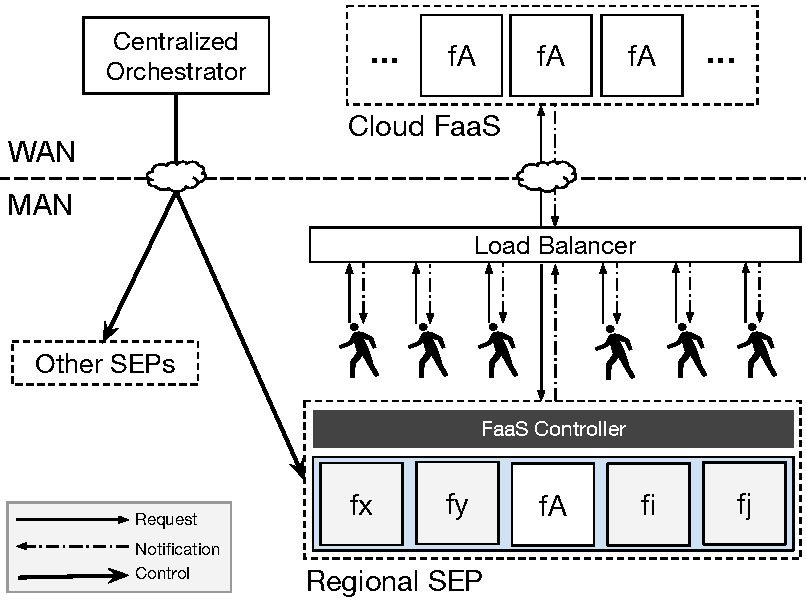
\includegraphics[width=0.97\linewidth]{Figs/Edge_Data_Analytics_Personal_Assistant.pdf}
	\caption{Nº of instances of the \textit{health analysis} function (fA) hosted by a Regional SEP is limited by a \textit{Centralized Orchestrator}; given the number of allocated instances, the latency requirements and the average response time, a \textit{Load Balancer} distributes requests among the SEP and the cloud-based FaaS.}
	\label{fig:Edge_Data_Analytics_Personal_Assistant}
\end{figure}

Going back to the AR example, Figure~\ref{fig:Mobile_Computation_Offloading_Workflow} depicts a simple workflow consisting of the sequential execution of the \textit{feature extraction} and \textit{matching} functions, which remain decoupled. In contrast with Figure~\ref{fig:Mobile_Computation_Offloading_F2}, both functions are served by the same SEP. A similar inter-platform cooperation could still be achieved with the delegation of requests coming from the \textit{Workflow Service} at one SEP to surrogate SEPs.

Last but not least, existing FaaS platforms (e.g., AWS Lambda~\cite{AWSLambda} and Apache OpenWhisk~\cite{OpenWhisk}) enforce a programming model in which functions have access to a transient container folder without guaranteeing that subsequent invocations will be handled by the same CER. %Thus, each invocation must check whether cached data is available. 
In the context of latency-sensitive applications, retrieving extensive data sets may add prohibitive overhead. For instance, in the AR example, a catalog (circa 1Gb) is used in the identification of points of interest (POI).
% against their matched features. 
Due to size limitations, it can not be packed with the function source code, but needs to be retrieved dynamically by each new CER instance.
%Cloud vendors provide storage services as part of their platform ecosystem. 

%TODO: make it consistent with the PROTOTYPE Section
%To address the need of edge services with dependency to large data sets
Addressing the aforementioned concern, we propose to equip SEPs with a \textit{Caching Service}. This service allows SEP functions to fetch data from the cloud and keep it available at the edge for mitigating networking overhead. 
%More precisely, the \textit{Caching Service} would consist of an object-based storage system (e.g., AWS S3), in which files are associated with metadata.  

%To make use of this service, SEP functions post a file passing its cloud \textit{URI}.
% which should return a valid file format.
% --- and an optional expiration policy. 
%The file is then stored along with metadata containing both its URI and the frequency of access. %subsequent requests are served with minimum overhead. 


The diagram in Figure~\ref{fig:Mobile_Computation_Offloading_Caching} depicts the interplay between a CER instance initialized with the \textit{feature matching} (fM) function and the \textit{Caching Service}.
Upon a first invocation, the fM function fetches a POI catalog (PC) from a cloud storage and adds it to the \textit{Caching Service} passing its cloud \textit{URI}. 
The file is then stored along with metadata containing both its URI and the frequency of access.
%and to its CER transient folder. 
Subsequent invocations handled by other CERs retrieve the cached file with a single request.
To cope with the limitation of storage resources, cached files are rotated according to their access frequency. %As such, files accessed less frequently are subject for been replaced in case of resource contention. 
%%Files without an expiration date are replaced only in case of resource contention following the access frequency policy. 
